\documentclass[12pt, onecolumn, a4paper]{exam}
\usepackage{amsmath}
\usepackage{amssymb}
\usepackage[lmargin=71pt, tmargin=1.2in]{geometry}  %For centering solution box
\lhead{TEK4090 -- Introduction to Modern Control\\}
\rhead{Assignment 3\\}
% \chead{\hline} % Un-comment to draw line below header
\thispagestyle{empty}   %For removing header/footer from page 1

\usepackage{graphicx}
\graphicspath{{./figures}}

\def\showsoln{1}

\begin{document}

\begingroup  
    \centering
    \LARGE TEK4090 -- Introduction to Modern Control\\
    \LARGE Assignment 4 v1.0\\[0.5em]
    \LARGE Part 1 of 3\\
    \large Due: December 5 2025, 23:30\\
\endgroup
\rule{\textwidth}{0.4pt}
%\pointsdroppedatright   %Self-explanatory
\printanswers


\renewcommand{\solutiontitle}{\noindent\textbf{Ans:}\enspace}   %Replace "Ans:" with starting keyword in solution box

\begin{questions}


\question[30] In this task, you will develop a mildly under-developed model-predictive control routine. The routine I am giving you has a bug, and you will have to figure out what I did wrong. Then, you will have to implement new modality into the code. The hard parts of this question are in (f), so make sure you give yourself enough time to do them.
  \begin{parts}
    \part For a prediction horizon of $k=0,\dots,T-1$, write the constraints
      \begin{align}
        z_0 &= \bar{z} \\
        z_{k+1} &= Az_k + Bu_k,\qquad k=0,\dots,T-1
      \end{align}
      in the form
      \begin{align}
        \Psi x - \Omega z_0 = 0
      \end{align}
      where
      \begin{align}
        x = \begin{bmatrix}
              z_1^T& \cdots&z_T^T & u_0^T & \cdots & u_{T-1}^T
            \end{bmatrix} ^T := 
        \begin{bmatrix}
          z\\u
        \end{bmatrix}
      \end{align}
    \part What cost function does the code encode?

    \part What system is the code trying to simulate, and does it have a name? What are the lower and upper bounds on the state and input constraints?

    \part Run the code. Note that it terminates due to an error at approximately $kk=14$. Debug the error, and describe what was happening. Plot the response of the system. Hint: look at the optimal control inputs and resulting states after propagating.

    \part How would you change the cost function in part  (b) to encode a penalty on the output $y_k=Cz_k$, instead of the state $z_k$? Would you changethe  constraint in part (a) as well?

    \part Notice that there is a $y^d$, or `desired trajectory' variable that is unused in line 29 or thereabouts. By using a quadratic penalty on $(y_l-y^d_k)$, re-write the debugged code so that the system tries to track this trajectory. You may find the following hints helpful:
      \begin{itemize}
        \item The desired trajectory is outside the system boundary. When you are close to the system boundary, process noise may push the system beyond the boundary, rendering the optimization problem infeasible and thus the code stops. This is bad. In order to fix this, you can use a `slack variable' $\sigma$ on the state $z_k$ dynamics constraint:
          \begin{align}
            \begin{bmatrix}
              -5 \\ -\infty
            \end{bmatrix} \leq 
            z_k \leq 
            \begin{bmatrix} 
              5 \\ \infty
            \end{bmatrix} \longrightarrow
            \begin{bmatrix}
              -5-\sigma_k^l \\ -\infty
            \end{bmatrix} \leq 
            z_k \leq 
            \begin{bmatrix} 
              5+\sigma_k^u \\ \infty
            \end{bmatrix} 
          \end{align}
          The point of $\sigma_i^{l,u}$ is that it is always zero, except when $z_k$ is close to the boundary. Then, if $z_k$ goes over the boundary, instead of the problem becoming infeasable, the system accrues some slack variable penalty. Therefore, you should also introduce an appropriate quadratic penalty on $\sigma$.
        \item To implement the slack variable, you will need to use the $A_{\text{ineq}}$ and $b_{\text{ineq}}$ entries of \texttt{quadprog}, and append the slack variable somehow to all the matrices that are entering quadprog:
          \begin{align}
            \begin{bmatrix}
              z \\ u
            \end{bmatrix} \longrightarrow
            \begin{bmatrix}
              z \\ u \\ \sigma^u \\ \sigma^l
            \end{bmatrix}
          \end{align}
        \item Right now, the linear part of the cost $f$ is zero. When you implement the desired trajectory by penalizing $(y_k-y_d^k)$, you will get a linear term when you expand the quadratic. This is what forms $f$. The constant term can be discarded, since a constant term isn't affected by the variable, and so discarding it doesn't change the optimizer.
      \end{itemize}
  \end{parts}

\begin{solution}
  \begin{parts}
    \part We know that the equation
    \[
        \begin{bmatrix}
            z_1 - Az_0 - Bu_0\\
            z_2 - Az_1 - Bu_1\\
            \vdots\\
            z_T - Az_{T-1} - Bu_{T-1}\\
        \end{bmatrix} = 0
    \]
    must be satisfied. We also have that. $ x = \begin{bmatrix}
        z\\ u
    \end{bmatrix} = \begin{bmatrix}
        z_1\\
        \vdots\\
        z_T\\
        u_0\\
        \vdots\\
        u_{T-1}
    \end{bmatrix}  $ where $ z_k \in \mathbb{R}^n $, $ u_k \in \mathbb{R}^m $  and thus, $ u \in \mathbb{R}^{nT}, u \in \mathbb{R}^{mT} $.We know furthermore that each row block enforces the eq
    \[
        z_{k+1} = Az_k + Bu_k
    \]
    The block matrix structure then becomes
    \[
        \phi_z = \begin{bmatrix}
            I&0 &\hdots& 0\\
            -A&I& & 0\\
            \vdots& & \ddots & 0\\
            0&0&0&I
        \end{bmatrix} 
    \]
    and 
    \[
        \Omega = \begin{bmatrix}
            A\\ 0\\ \vdots\\ 0
        \end{bmatrix}  \in \mathbb{R}^{nT\times n}
    \]
    
    If we for verification place K=3 we get that the equation

    \[
        \Psi x - \Omega z_0 = 0
    \]
    indeed becomes true

    \begin{align*}
      \begin{bmatrix}
            1&0&-B&0\\
            -A&1&0&-B
        \end{bmatrix} \begin{bmatrix}
            z_1\\
            z_2\\
            u_0\\
            u_1
        \end{bmatrix}   - \begin{bmatrix}
            A\\ 0
        \end{bmatrix} z_0 &= \begin{bmatrix}
            z_1 - Bu_0 - Az_0 \\
            -Az_1 + z_2 -Bu_1 
        \end{bmatrix} =0 \\
        \rightarrow \begin{bmatrix}
            z_1\\ 
            z_2
        \end{bmatrix} = \begin{bmatrix}
            Az_0 + Bu_0\\ Az_1 + Bu_1
        \end{bmatrix}  
    \end{align*}

    \part The cost function that the code is encoding is 
    \[
        J = \sum_{ k=1 }^{ T } z_k^TQz_k + \sum_{ k=0 }^{ T-1 } u_k^TR u_k
    \]
    

    \part The system that the code is trying to simulate is the discrete time LTI double integrator system with a gaussian process and measurement noise. The states are position and velocity, while the inputs are acceleration. The output is the position

    \part

    I have made a figure that plots the velocity, position and the input u right before the error in the code ocurred.
    \begin{center}
      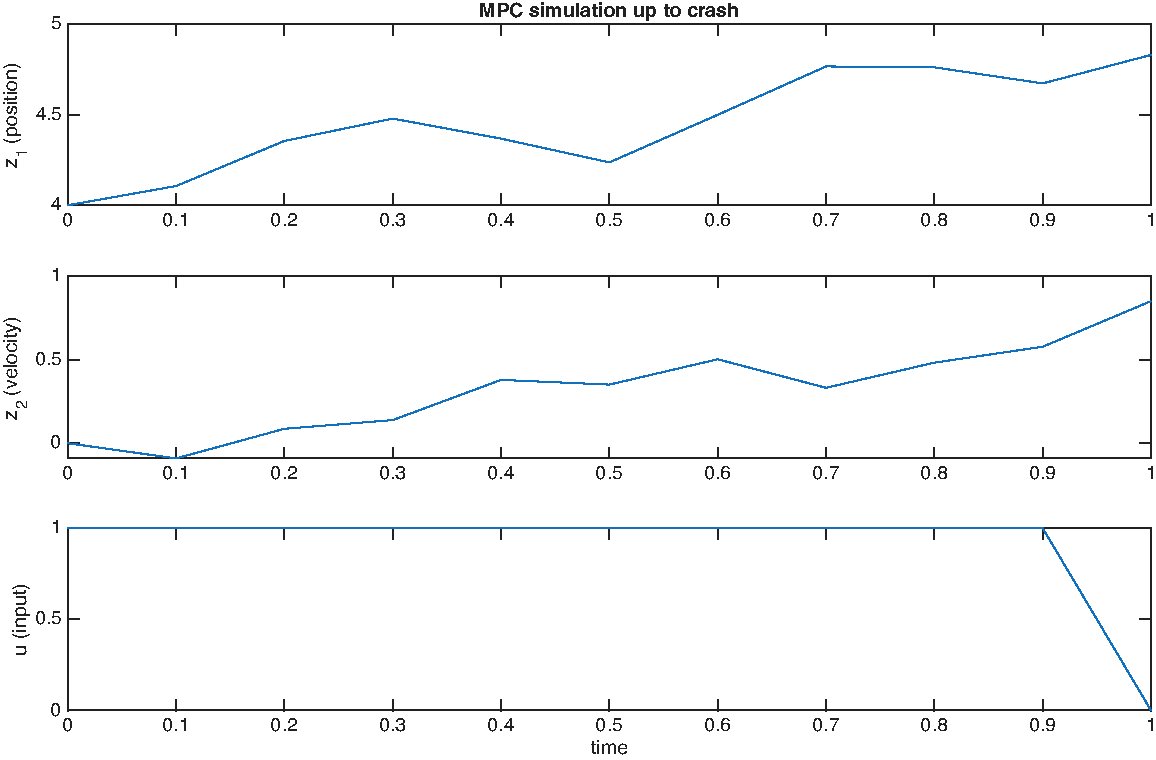
\includegraphics[width = 1\linewidth]{debug_1d.pdf}
    \end{center}

    The code fails because the MPC QP problem becomes infeasible. Whats happening here is that the position $ z_1 $ is pushed outside of its domain $ \left[ -5, 5 \right] $. Given the input constraints and disturbances, there is no control sequence that can keep the position inside the bounds $ \left[ -5, 5 \right]  $. This is why the code stops after cirka 14 iterations, because the QP has no feasible solution and the quadprog returns an error which causes the loop to stop. The control signal shows that its reached its limit before the loop stops, which explains why the controller cant keep the position within its bounds.


    \part To penalize the output, we replace the cost function
    \[
        J = \sum_{ k=1 }^{ T } z_k^T Q z_k + \sum_{ k=0 }^{ T-1 } u_k^T R u_k
    \]
    with $ y_k = C z_k $
    \begin{align*}
      J &= \sum_{ k=1 }^{ T } \left( C z_k \right)  ^T Q \left( C z_k \right)  + \sum_{ k=0 }^{ T-1 } u_k^T R u_k \\
      &= \sum_{ k=1 }^{ T } z_k^T  \left( C^T  Q C \right)  z_k + \sum_{ k=0 }^{ T-1 } u_k^T R u_k
    \end{align*}
    The constraints will remain the same. The MPC used to track the states, and now we track the output instead

    \part Here is a plot of the implemented code

    \begin{center}
      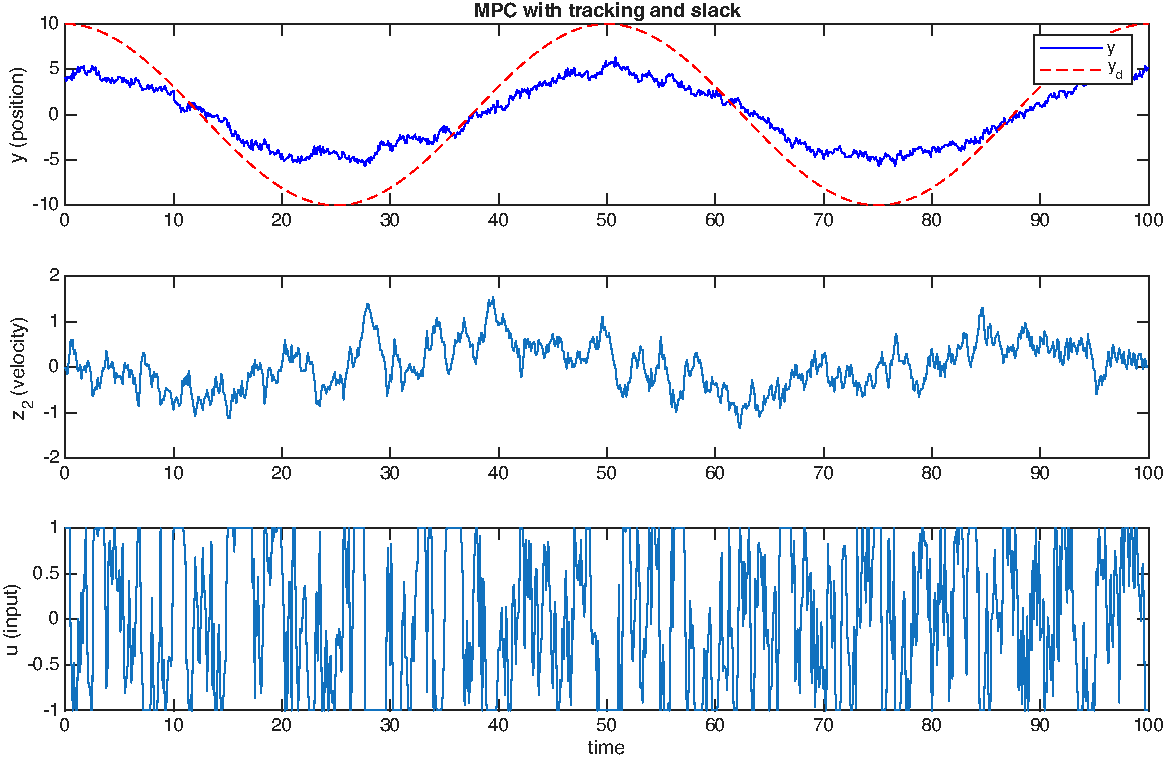
\includegraphics[width = 1 \linewidth]{part5_plot.pdf}
    \end{center}

    This does a much better job at tracking the sinusoidal reference that was defined in line 29 of the code. 

    When we introduced the reference tracking $ y_k - y^d = C z_k - y_d $ we got that the expression $ \left( C z_k - y_k^d \right)^T Q_y \left( C z_k - y_k^d \right)   $  expanded to a quadratic, a linear and a constant term. We dropped the constant term from the function becuase its irrelevant to optimization, and got 
    \[
        J = \sum_{ k=1 }^{ T } z_k^T C^T Q_y C z_k - 2 (y_k^d)^T Q_y C z_k + \sum_{ k=0 }^{ T-1 } u_k^T R u_k = 
    \]
    where $ Q_y = 1 $, this is because $ C = \begin{bmatrix}
        1\\ 0
    \end{bmatrix}  $ and $ y_k = Cz_k = \begin{bmatrix}
        1\\ 0
    \end{bmatrix} z_k =z_{1,k}  $. Therefore
    \[
        C^T Q_y C = \begin{bmatrix}
            1&0\\ 0&0
        \end{bmatrix} 
    \]. The first term acts as a quadratic penaly on $ z_{1,k} $ . The second linear term $ -2 y_k^d z_{1, k} $ is important because its what makes the MPC follow the time varying reference. If we dont include this term, the controller would simply drive the position state toward zero rather than track $ y_k^d $ 
     
     
    

  \end{parts}
\end{solution}

\end{questions}




\end{document}